\chapter{Data Analysis}\markboth{Data Analysis}{}

% \section{Signal Interpretation}

    To produce meaningful results from the raw data taken in the experiment, some data processing is necessary. The 'raw' information gathered by the detectors is in the form of a voltage waveform, as seen for example in figure \ref{fig:waveform-real}. Each of the eight \ac{SiPM}-groups, as well as each of the \acsp{PMT}, records one such waveform for each event.
    
    \begin{figure}[h]
    	\centering
    	\begin{subfigure}{.5\textwidth}
    		\centering
    		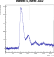
\includegraphics[width=.7\textwidth]{pictures/waveform-sipm.pdf}
    		\caption{}
    		\label{fig:waveform-sipm}
    	\end{subfigure}%
    \begin{subfigure}{.5\textwidth}
    	\centering
    	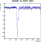
\includegraphics[width=.7\textwidth]{pictures/waveform-pmt.pdf}
    	\caption{}
    	\label{fig:waveform-pmt}
    \end{subfigure}
	\caption{Waveforms recorded from an arbitrarily chosen event. a) Waveform recorded in \ac{SiPM} group connected to channel 0. b) Waveform recorded in \ac{PMT} connected to channel 10.}
	\label{fig:waveform-real}
    \end{figure}

	The \ac{SiPM} waveform can be roughly separated into three intervals, clearer to be seen in figure \ref{fig:waveform-sum}:
	The first region, ranging from the start of the waveform to its rising edge, is the one \textit{without a main signal}. This interval mainly consists of effects of \ac{SiPM} and electronic noise and \ac{DC} events, as well as muons, which crossed the \ac{LS} detector box, but not the plastic scintillators. As it should fluctuate around zero, it is also used to calculate the systematic offset from zero that is measured in the detectors, the so-called baseline.
	The \textit{rising edge} describes the steep increase in voltage as the silicon photodetectors detect scintillation photons. Its slope varies, depending on the arrival time of registered photons. 
	The rising edge culminates in the peak of the signal shape, at which point the voltage starts to drop again, forming the \textit{falling edge}. Ideally, this edge would decrease until it reaches the starting levels of noise again, however in reality,  this is not the case. The waveform recorded by a group of \acsp{SiPM} is a superposition of signals measured in the five singular ones that build the group. It is therefore broader but smoother than a single-\ac{SiPM} waveform - an effect we can 'amplify' by regarding the sum of waveforms for several events, as was done in \ref{fig:waveform-sum}. After the falling edge, the voltage does not drop to baseline levels, but shows after-peak oscillations, which are likely caused by an impedance difference between the signal transmitting cables, the eMUSIC board and the WaveCatcher \cite{ZACHARIAS}. They are not part of the main signal stemming from scintillation photons, which will be considered in the data analysis.
	
	
	
	
	\begin{figure}[h]
		\centering
		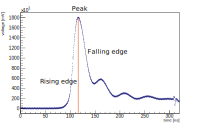
\includegraphics[width=.7\textwidth]{pictures/waveform-sum.pdf}
		\caption{Sum of waveforms for arbitrary run and channel (here: channel 0), summing about \num{70000} events. The flat first region is dominated by noise and \ac{DC} events, followed by the main signal peak and after-peak oscillations.}
		\label{fig:waveform-sum}
	\end{figure}
    
    

\section{RootReader}

	The WaveCatcher signal processing software stores the converted digital data in binary files, with about 500 events per file, each event consisting of 12 voltage waveforms with a time span of 320ns each. With each run totalling around 70000 events to be analysed, this results in a high number of binary files, taking up a lot of storage space. This problem however has been addressed before \cite{HANEL}, and the data analysis for this experiment was once again completed using an adapted form of the RootReader software routine developed by Jan Zimmerman \cite{ROOTREADER}. This routine, written in C++ and based on the ROOT framework provided by CERN \cite{CERN}, reduces required storage space by concentrating the information held in the binary files to useful variables only, for example the pulse height and timing, calculated by the routine itself. It then stores these variables in ROOT-files, which take up less storage space and can be easily accessed for further analysis. It is also during this conversion to ROOT files that events can be selected or cut on desired conditions. The filtered events are saved in a so-called \lstinline|Tree|-structure, in which calculated variables are grouped together in \lstinline|Leaves| and can then be easily presented in histograms. Further analysis and plotting was then done in C++ as well as python. 
    The main characteristics of an event considered in this thesis are its light yield and the location of the muon crossing the detector box.

\section{Light Yield}

    To explore the detector's response to different scintillation light source locations, we need to be able to compare the amount of light reaching the different \acsp{SiPM} groups making up the detector.
	An incident photon on a \ac{SiPM} pixel will cause a current $I(t)$ in this pixel, measured by the readout electronics as a change in voltage $U(t)$. Integrating this voltage over the time interval $\Delta t$ it occurred in gives us a measure for the charge $Q$ resulting from the photon:
	
% 	Formula: Integral I(s) ts over Signal, 1/R U(t) over signal
	\begin{align}
	    Q =  \int_{\Delta t} I(t) \,dt = \frac{1}{R} \int_{\Delta t} U(t) \,dt 
	\end{align}
	
	
	Since the charge created during an event is dependent on the number of scintillation photons produced by the crossing particle, the integral of the voltage waveform will also be called the 'light yield' in this thesis. The actual amount of overall photoelectrons produced in an event could then be calculated from the light yield of all \acsp{SiPM} together, however for this one would need calibration data for the specific \ac{PCB} used in the experiment, which was not available here. 
	For this thesis however this was not necessary, as one can still compare the light yield of the \acsp{SiPM} between different runs, without knowing the actual number of photoelectrons created. The light yield $J$ will therefore be given in units of \SI{}{\volt\nano\second} and not converted to units of charge.
%	\todo{Integration window calculation more}
	To determine the integration time window for one channel, the sum of all waveforms of all events in this channel was used.  Only the 'main' signal was considered, with the integration window starting \SI{20}{\nano\second} before the signal's peak value, and reaching until the first minimum before the after peak oscillations (see figure \ref{fig:integration-window}).
	
	\begin{figure}[h]
		\centering
		\includegraphics[width=.8\textwidth]{pictures/integration-window.pdf}
		\caption{The summed up waveforms in one channel of about \num{70000} events added together. The outer orange lines mark the integration window, the inner one the amplitude of the peak.}
		\label{fig:integration-window}
	\end{figure}
	
	The RootReader routine determines one unique integration window size for each \ac{SiPM} group channel, that is then applied relative to the reference point, the signal peak, for each event \cite{ZIMMERMANN}.
	The light yield is also used to set a threshold for cutting out \ac{DC} events: In earlier experiments' measurements with this prototype detector, it was determined that these have a significantly lower number of photoelectrons than non-\ac{DC} events do \cite{HANEL,ZACHARIAS}. Additionally, it can be used to cut out events that are unlikely to be caused by a single muon, as they show significantly higher light yields than expected. For all data sets analysed in this thesis, the light yield interval allowed was set to be 300 to \SI{1500}{\volt\nano\second}. 
	
%	FIGURE: waveform with integration windows, asymmetry marked


\section{Positional Data}\label{sec:positional-data}

    To determine the positional dependence of the detector's response, it is of course necessary to be able to correlate its response with the known location of an incident particle.
	For this, two plastic scintillators were used, located beneath and on top of the detector box, as described in chapter \ref{cosmics}.
	Their scintillation light was collected by two \acsp{PMT} each, for a total of four photodetectors.
	Since the total distance between two \acsp{PMT} in a set was static, one could then calculate the position of a crossing particle on the \ac{PS} from the timing of the signals measured in the two \acsp{PMT}.
	For this, the speed of light inside the plastic scintillator is needed: This we can calculate using the refraction index $n$ of the scintillating material, which is about $n = 1.5$ \cite{ZACHARIAS}. However, inside the plastic scintillator, the light will hardly ever reach a \ac{PMT} in a straight path, but rather get reflected many times at the surfaces, increasing the time before the signal gets detected. This we can express by additionally reducing the speed of light $c$ by a factor $f_{refl.}$, resulting in typical values of an effective speed of light of:
	\begin{align}
	    c_{PS} = \frac{1}{n} \cdot f_{refl.} \cdot c \simeq \frac{1}{2} \cdot c = \SI{15}{\centi\meter\per\nano\second}
	\end{align}
	
	With the detector box being $L = \SI{50.4}{\centi\meter}$ in width, this means that a particle that crosses at one corner of the scintillation box would cause scintillation light in the plastic scintillators that would take about $t = \frac{L}{c_{PS}} = \SI{3.3}{\nano\second}$ to reach the other side of the detector.
	Since the light in the \ac{PS} will distribute in all directions and get picked up separately by the two \ac{PMT} at either end, due to the difference in travel lengths, we can use this time difference to determine where along the \ac{PS} the scintillation light was generated.
	Calling the times measured at either \ac{PMT} $t_1$ and $t_2$ respectively (see figure \ref{fig:time-difference}), the distance $X_{top}$ from the middle of the \ac{PS} can be determined using the difference $\Delta t_{12}$ as follows:
	\begin{align}
	    X_{top} = \frac{1}{2} \cdot c_{PS} \cdot (t_2 - t_1) = \frac{1}{2} \cdot c_{PS} \cdot \Delta t_{21}
	    \label{eq:timing}
	\end{align}
	
	Here, if $X_{top} < 0$, it lies to the right of the centre point, if $X_{top} > 0$, it lies to the left.
	Doing this for both \ac{PS}, we can now reject events if they do not stem from a particle passing through the detector box in a certain area.
	For \ac{PMT} 3 and 4, the same principles hold, so in the bottom \ac{PS} we can also determine distance $X_{bot}$ from the centre using $X_{bot} =  \frac{1}{2} \cdot c_{PS} \cdot (t_4 - t_3) = \frac{1}{2} \cdot c_{PS} \cdot \Delta t_{43}$.
	Now accepting only events that have, for example both $X_{top}$ and $X_{bot}$ in a certain interval around 0, we allow only events stemming from a muon passing roughly through the centre of both \ac{PS}. For this, we restrict $\Delta t_{21}$ and $\Delta t_{43}$ to result in the desired $X$-values. 
	The accuracy of this positioning of course depends on the time resolution of each of the \ac{PMT}s.
	
	\begin{figure}[h]
		\centering
		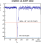
\includegraphics[width=.4\textwidth]{pictures/cfd.pdf}
		\caption{A \ac{PMT} waveform from arbitrarily chosen events. Marked are the minimum of the peak, and the muon arrival time, calculated via \ac{CFD} with a threshold of \num{0.5}.}
		\label{fig:CFD}
	\end{figure}

	For the analysis, 9 positions were defined as documented in table \ref{tab:positions} and illustrated in figure \ref{fig:locations-cosmics}. The capital letters indicate the positions of the plastic scintillator to the left (L), right (R) and on top (C) of the \ac{WOM}, which is located in the middle of the detector box. An example of a cut can be seen in figure \ref{fig:timing-cut}. Here, the first plots show the time differences $\Delta t_{21}$ and $\Delta t_{43}$ of a run of about \num{70000} events, and the lower plots show the $\Delta t_{21}$ and $\Delta t_{43}$ diagrams for the same run, where only events corresponding to position R-0 have been allowed. 
	
	\begin{figure}[h]
		\centering
		\begin{subfigure}{\textwidth}
			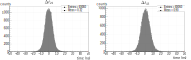
\includegraphics[width=\textwidth]{pictures/time-differences-uncut.pdf}
			\caption{Time differences measured in \acsp{PMT} for run with about \num{70000} events. There was no fit done here, as the distribution is a convolution of a uniform (due to the muons crossing the scintillators in no preferred location) and a Gaussian (due to the smearing of measured arrival times) distribution.}
			\label{fig:timing-nocut}
		\end{subfigure}
		\begin{subfigure}{\textwidth}
			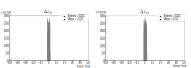
\includegraphics[width=\textwidth]{pictures/time-differences-cut.pdf}
			\caption{Time differences measured in \acsp{PMT} for the same run as above, but with a cut applied. Only events in position R-0 were allowed, all others rejected.}
		\end{subfigure}
	\caption{Time differences $\Delta t_{21}$ and $\Delta t_{43}$ for a run with a) no cuts applied and b) for position R-0.}
	\label{fig:timing-cut}
	\end{figure}
	
	The arrival time $t_a$ of the crossing muon was determined using \ac{CFD}, a method that determines the position of a pulse's peak, independent of the peak's height. For all four \acsp{PMT}, the threshold for the \ac{CFD} was set to \num{0.5}, meaning the arrival time was found, when the measured voltage reached \SI{50}{\percent} of its minimum, as is illustrated in figure \ref{fig:CFD}. 
	
	
	
% 	TABLE positions
	\begin{table}[h]
	\centering
    \begin{tabular}{@{}lll@{}}
    \midrule
    Position & $\Delta t_{21} (\SI{}{\nano\second})$ & $\Delta t_{43} (\SI{}{\nano\second})$ \\ \midrule
    C,L,R-0  & {[}-1.75, 2.25{]}                     & {[}-1.15, 2.85{]}                     \\
    C,L,R-1  & \textgreater{} 6.25                    & \textgreater{} 6.85                    \\
    C,L,R-2  & \textless{} -5.75                      & \textless{} -5.15                      \\ \midrule
    \end{tabular}
    \caption{Time difference cuts for positions chosen for analysis, as illustrated in figure \ref{fig:locations-cosmics}.}
    \label{tab:positions}
    \end{table}
	
	Like this, position C-0 for example lies in the centre of the detector box, as seen in the schematic in figure \ref{fig:locations-cosmics}. The positions were chosen to accommodate for clear spatial differences between them, while keeping a reasonable number of events in each cut for statistics.
	

	\begin{figure}[h]
		\centering
%		\todo[inline]{maybe adjust relative measurements}
		\begin{subfigure}{.5\textwidth}
			\centering			
			\includegraphics[width=\textwidth]{pictures/positional.pdf}
			\caption{}
			\label{fig:time-difference}
		\end{subfigure}%
		\begin{subfigure}{.5\textwidth}
			\centering
			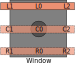
\includegraphics[width=.7\textwidth]{pictures/locations_cosmics.pdf}
			\caption{}
			\label{fig:locations-cosmics}
		\end{subfigure}	
	
	\caption{a) Schematic of cosmics setup with four \acsp{PMT} (blue), two \ac{PS} (orange) and the detector box (grey) as seen when viewed from the laboratory's window. A muon crossing the setup (dashed line) can be located using the timing data taken by the \acsp{PMT}. b) Schematic top view of the cosmics setup illustrating the approximate muon crossing locations chosen to be analysed. The second plastic scintillator would be located directly underneath the one seen in the illustration (opaque orange), meaning the muon crossed parallel to the covered \ac{WOM} (dark-grey) through the detector box. The set of two \ac{PS} would then get pushed together, to reach the other positions (translucent orange). }	
	\end{figure}

\section{Time Resolution of the Plastic Scintillators}

The positional cuts of muon events were done using timing data taken by four \acsp{PMT} located above and below the detector box, as described in section \ref{sec:positional-data}. The detector box is about \SI{50.4}{\centi\meter} wide, which translates to a maximum absolute time difference $\Delta_{21}$ and $\Delta_{43}$ of about \SI{3.3}{\nano\second} (plus some smearing due to the time resolution of the \acsp{PMT}) we should see in the time difference distributions for the measurement runs. As visible in figure \ref{fig:timing-nocut}, however, the distribution is a lot wider than this. This lead us to suspect the time resolution of the \acsp{PMT} to be worse than expected, which is why an attempt to quantify it was made.

%	FIGURE time dif plots top and bottom

The time resolution was estimated by calculating the value $(t_1 + t_2 - t_3 - t_4)/4$, which is the average time of flight between the two \ac{PS} of a particle triggering a measurement, divided by \num{2}. 
Considering only particles passing straight through the centre of the detector box, the average time of flight should stay the same for all events, since diagonal paths are cut out.
This means that the width of the distribution of $\frac{1}{2}\cdot (t_1 + t_2 - t_3 - t_4)/2$ would give a measure for the average time resolution of all four \acsp{PMT}. The factor $\frac{1}{2}$ is added as one has to consider a time with the same factor as the mean time of arrival measured by all \acsp{PMT}: $(t_1 + t_2 + t_3 + t_4)/4$.
An example of the $(t_1 + t_2 - t_3 - t_4)/4$ distribution is given in figure \ref{fig:time-resolution}. The time resolution of the \acsp{PMT} in this setup was thereby found to be about \SI{1}{\nano\second}. % and taken into consideration when applying positional cuts by allowing a wider range of time differences measured in one position than one would calculate from formula (\ref{eq:timing}). 

However even taking into account a $\pm \SI{1}{\nano\second}$ uncertainty, the width of the delta t distribution in \ref{fig:timing-nocut} is higher than the expected \SI{3.3 \pm 1}{\nano\second}. 

%    FIGURE time resolution 
\begin{figure}[h]
	\centering
	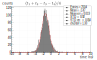
\includegraphics[width=.7\textwidth]{pictures/time-resolution.pdf}
	\caption{Time of flight distribution for position R-0, divided by 2. }
	\label{fig:time-resolution}
\end{figure}

To check for consistency in the \ac{PMT} measured arrival times, we can calculate the mean flight time of a muon between the plastic scintillators by multiplying the mean value of the $(t_1 + t_2 - t_3 - t_4)/4$ by 2 again. This value, when multiplied by the velocity of the muons, should match the distance between the two plastic scintillators. Approximating the muons' velocity with the speed of light to $c = \SI{3e08}{\meter\per\second}$ we get a distance of about $ c \cdot 2 \cdot \SI{1.47}{\nano\second} \simeq \SI{0.88}{\meter}$, which is slightly higher than the real distance of about \SI{66}{\centi\meter}. Since this time however should be quite constant for all events in the cut, the width of this peak appears very wide as well. 
As this remained unexplained, and a great number of events in a run lie outside of the expected \SI{3.3 \pm 1}{\nano\second} interval, the positional cuts were extended in width from what one would expect from formula (\ref{eq:timing}), to keep a reasonable number of events. 





\section{Event-dependent Mean Angle \texorpdfstring{$\phi_{ew}$}{}}

	The goal of this thesis is to explore the location dependent response of the \ac{LS} prototype detector and compare it to earlier experiments. 
	For this, a value $\phi_{ew}$ was introduced and calculated as previously done by Joscha Hanel in his bachelor's thesis \cite{HANEL}.
	To compare the detector response between different events, an estimator is used, that, for each event separately, represents the channel in the \ac{WOM} \ac{SiPM} Array, where the scintillation light was picked up.
	In reality of course, all 8 channels would detect a signal from one event, meaning there is no singular channel that picked up the scintillation light. 
	This is where the mean angle $\phi_{ew}$ is introduced:
	Every channel $i \in [0,7]$ in the \ac{SiPM} detector array was assigned an angle $\varphi_i$ between 0 and 360° as shown in figure \ref{fig:channel-phi}.
	
	\begin{figure}[h]
		\centering
		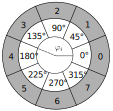
\includegraphics[width=.3\textwidth]{pictures/phi_channel.pdf}
		\caption{Schematic of \ac{SiPM} channels. Each of the 8 channels (numbered 0 to 7) was assigned an angle $\varphi_i$, that was then used to calculate the mean angle $\phi_{ew}$.}
		\label{fig:channel-phi}
	\end{figure}
	
	This angle is then weighed by the light yield $J_{i}$ measured in this channel and contributes to the overall average of these angles.
	Just averaging the angles directly would not make sense however: The average of 0° and 180° being 90° would imply most photons reached the channel with 90° assigned to it, when in reality they were just evenly distributed to two opposite sides.
    For this reason, the average was handled as a vectorial addition: 8 polar vectors with the angle assigned to the channel and a length set to the measured light yield were added together, and interpreted as a new polar vector with the 'mean' angle $\phi_{ew}$:
    
    \begin{gather}
    	\begin{align*}
    		x_{i}& = \cos(\varphi_{i}) \cdot J_{i} 
    		& y_{i} &= \sin(\varphi_{i}) \cdot J_{i}\\
    		X  &= \sum_{i=0}^{7} x_{i}
    		& Y &= \sum_{i=0}^{7} y_{i}\\
    	\end{align*}
     \end{gather} 
    	
    	The conversion back to a polar angle then gives:
    	
    	\begin{align}
    		\label{eq:phiew}
    		\phi_{ew} = \arctan\qty(\frac{Y}{X})
    	\end{align}
    

\chapter{Results and Discussion}\markboth{Results and Discussion}{}

    For each of the three plastic scintillator positions (C, L, R), runs with \num{70000} to \num{90000} events were recorded over the course of several days each, all during daylight hours. During this time, the temperature in the laboratory was kept under observation, as the \acsp{SiPM} response varies with fluctuations in the temperature. The mean temperature for the run used for positions L-0,1,2 was about \SI{24.01}{\celsius}, the one for C-0,1,2 about \SI{23.62}{\celsius}, and the one for R-0,1,2 about \SI{23.42}{\celsius}. The temperatures fluctuated by around \SI{0.4}{\celsius} to \SI{0.7}{\celsius} over the course of each run. As the light yield was not converted to photoelectric charge and only compared within runs, thereby not necessitating calibration values, adjustments in the conversion from light yield to photoelectric charge due to the small fluctuations in temperatures were not necessary.
    The results of the analysis of the events collected in the measurement runs are presented and discussed in this chapter.

\section{Position-dependent Mean Angle \texorpdfstring{$\overline{\Phi_{ew}}$}{}}

	
	The $\phi_{ew}$ distribution for an example run and position, here position R-0, is shown in figure \ref{fig:phi-ew-R0}. The distribution has a periodicity of \SI{360}{\degree} due to the nature of the variable, but was plotted over an interval of \SI{-180}{\degree} to \SI{180}{\degree}  for better peak visualisation and comparison with previous experiments. The location of the peak is given relative to channel 0, which was assigned the $\varphi_i$ value \SI{0}{\degree}. This means, that the peak at \SI{40}{\degree} implies that the mean photon impact was detected closer to channel 1, which has the assigned angle of \SI{45}{\degree}.
	
	\begin{figure}[h!]
	    \centering
	    Mean angle $\phi_{ew}$ for position R-0, relative to ch. 0
	    \includegraphics[width=.9\textwidth]{pictures/phi_ew_R0.pdf}
	    \caption{Mean angle $\phi_{ew}$ distribution for position R-0. The $\phi_{ew}$ values are given relative to ch. 0 at $\phi_{ew} = 0$. Each bin represents an angle interval of \SI{2}{\degree}.}
	    \label{fig:phi-ew-R0}
	\end{figure}
	
	As visible in figure \ref{fig:phi-ew-R0}, the normal distribution of $\phi_{ew}$ values in reference to channel 0 viewed over this interval is not centred around 0, and therefore not easily fitted, without already knowing by how many degrees the entire distribution is shifted. 
	As mentioned above, however, the $\phi_{ew}$ values are periodic with a periodicity of \SI{360}{\degree} degrees, a fact which was used in the determination of the actual mean values of each distribution:
	The distribution was inserted three times into a histogram, one time without a shift in values, and once shifting the values by \SI{\pm 360}{\degree}, respectively.
    This results in a plot such as figure \ref{fig:3-phi-ew-R0}, with three peaks. With the knowledge that all peaks must have the same height, width and, except for the shift by 360°, position, we can now fit a combination of three Gaussians to the distribution:
    
    \begin{multline}
        f_{3G} = p_0 \cdot \left[\exp(-\frac{1}{2}\qty(\frac{x-p_1+360}{p_2})^2) + \exp(-\frac{1}{2}\qty(\frac{x-p_1}{p_2})^2) \right. \\ 
        \left. + \exp(-\frac{1}{2}\qty(\frac{x-p_1-360}{p_2})^2)\right] + p_3
    \end{multline}
    
    The initial fit parameters were set by calling the ROOT methods \lstinline|TH1F:GetMaximum()|, \lstinline|TH1F:GetRMS()| and \lstinline|TH1F:GetMean()| on the histogram containing only one peak, the fit itself was also done using the appropriate ROOT methods.
    The mean value $\overline{\Phi_{ew}}$ of the $\phi_{ew}$ distribution was now obtained from the fitted triple-Gaussian: $ \overline{\Phi_{ew}} = p_1$. Its standard deviation is $\sigma = p_2$. Values $p_0$ and $p_3$ are the height of the peak and the minimum value of the function respectively, but were not used in further analysis.
    
    \begin{figure}[h!]
        \centering
        Mean angle $\phi_{ew}$ for position R-0, shifted by 0 and \SI{\pm 360}{\degree}
        \includegraphics[width=.9\textwidth]{pictures/phi_ew_R0_shift.pdf}
        \caption{Mean angle values for position R-0, shifted by 0 and $\pm$ \ang{360} to enable easier fitting. The $\overline{\Phi_{ew}}$ is the position of the middle peak, $\sigma$ its standard deviation.}
        \label{fig:3-phi-ew-R0}
    \end{figure}
    
    Gathering the $\overline{\Phi_{ew}}$ values for the 8 positions, omitting position C-0, we can now compare the detector's response to different locations of particle interaction. Position C-0 is omitted, since, in theory, for this position particles are going through the middle of the \ac{WOM}, which should result in a uniform distribution of $\phi_{ew}$ angles. This position was therefore left out here, and analysed separately.

    
    Naively, one would expect the $\overline{\Phi_{ew}}$ to be evenly distributed on a circle, each angle corresponding to the direction in which the muon crossed the scintillators. To visualise this, we calculated an angle $\alpha$ for each of the positions, as seen in table \ref{tab:muon_angles}. Viewing the $\overline{\Phi_{ew}}$ as dependent on their respective $\alpha$ we would then expect a more or less linear relationship.
    
%    \begin{table}[h]
%        \centering
%        \begin{tabular}{@{}lll@{}}
%        \midrule
%           Position  &  Muon angle $\alpha$ (\SI{}{\degree}) \\
%           \midrule
%           C-2          &   0 \\
%           L-2          &   32.89\\
%           L-0          &   89.95\\
%           L-1          &   151.83\\
%           C-1          &   180\\
%           R-1          &   208.17\\
%           R-0          &   270.05\\
%           R-2          &   327.11\\
%        \midrule
%        \end{tabular}
%        \caption{Caption}
%    \end{table}
    
\begin{figure}[h!]
\begin{floatrow}
\capbtabbox{%
  \begin{tabular}{@{}lll@{}}
        \midrule
           Position  &  Muon angle $\alpha$ (\SI{}{\degree}) \\
           \midrule
           L-0          &   +123 \\
           L-2          &   +66\\
           C-2          &   +33\\
           R-2          &   0\\
           R-0          &   -57\\
           R-1          &   -119\\
           C-1          &   -147\\
           L-1          &   -175\\
        \midrule
        \end{tabular}
    }{%
        \caption{Muon angles assigned to a measurement position. The angles were chosen so that $\overline{\Phi_{ew}} = \ang{0}$ relative to channel 0 matches $\alpha = \ang{0}$.}
        \label{tab:muon_angles}
    }
    \ffigbox{%
        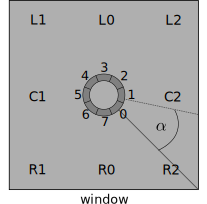
\includegraphics[width=.45\textwidth]{pictures/relative-locations.pdf}
    }{%
         \caption{Relative positioning of \ac{SiPM} channels in \ac{LS} box.}%
         \label{fig:muon_angles}
}
\end{floatrow}
\end{figure}

%\begin{table}[h]
%	\begin{tabular}{@{}lll@{}}
%		\midrule
%		Position  &  Muon angle $\alpha$ (\SI{}{\degree}) \\
%		\midrule
%		C-2          &   0 \\
%		L-2          &   32.89\\
%		L-0          &   89.95\\
%		L-1          &   151.83\\
%		C-1          &   180\\
%		R-1          &   208.17\\
%		R-0          &   270.05\\
%		R-2          &   327.11\\
%		\midrule
%	\end{tabular}
% 	\caption{Muon angles assigned to a measurement position. Angles for position C-1 and C-2 were not calculated but defined as the reference points.}
%    \label{tab:muon_angles}
%\end{table}



    
    The $\overline{\Phi_{ew}}$ as viewed in dependence of the muon angle $\alpha$ is visible in the upper plot in figure \ref{fig:phi-ew-alpha}.
    
    \begin{figure}[h!]
        \centering
        \includegraphics[width=\textwidth]{pictures/phi-ew-std-sep.pdf}
        \caption{Mean angles $\overline{\Phi_{ew}}$ (top) with their standard deviations $p_2 = \sigma$ as error bars, and the standard deviations $p_2 = \sigma$ (bottom) in dependence of the muon incidence location, expressed as $\alpha$.}
        \label{fig:phi-ew-alpha}
    \end{figure}
    
    % FIGURE $\overline{\Phi_{ew}}$ angles muon angles normal, center 0
    
   

    
    % FIGURE $\overline{\Phi_{ew}}$ phi-ew angles  radial, center 0
    
    One is quick to notice that the $\overline{\Phi_{ew}}$ values do not span over the entire \SI{\pm 180}{\degree} interval we might have expected, but only take up about a quarter of it, more easily visible in figure \ref{fig:phi-ew_polar}. 
    We do not necessarily expect the muon angle to directly match the $\overline{\Phi_{ew}}$ value, as the light in the \ac{WOM} tube is likely not transported directly towards a \ac{SiPM}, but rather in a spiral-shaped path, caused by the internal reflections off the \ac{WOM}'s walls, meaning while we expected a linear $\overline{\Phi_{ew}}$ - $\alpha$ relationship, all values could be shifted by some degree.
    The assumption that they should span the circle is of course dependent on a perfect optical coupling and alignment between the \ac{WOM} tube and the \ac{SiPM} array. This, however, is not guaranteed as there are several different types of material connecting the two, influencing the transmission of wavelength-shifted light. Furthermore, it is likely that for each channel, there is a slight difference in combination of materials, for example a variation in the thickness of optical gel. All this means of course, that the exact optical coupling is unique for an experimental setup, and would have to be studied again if one would change said setup.
    
     \begin{figure}[h!]
    \centering
    \begin{subfigure}{.5\textwidth}
      \centering
      \includegraphics[width=\textwidth]{pictures/phi-ew-radial.pdf}
      \caption{$\overline{\Phi_{ew}}$, radial view.}
      \label{fig:phi-ew_polar}
    \end{subfigure}%
    \begin{subfigure}{.5\textwidth}
      \centering
      \includegraphics[width=\textwidth]{pictures/locations.pdf}
      \caption{Measurement locations on the detector box.}
      \label{fig:locations}
    \end{subfigure}
    \caption{$\overline{\Phi_{ew}}$ values in a polar plot, given relative to channel 0. The angle \SI{0}{\degree} corresponds to channel 0, as indicated by the numbers in the inner circle of plot a). Each symbol-colour-combination stands for one measurement position, illustrated in plot b).}
    \label{fig:phi-ew}
    \end{figure}
    
    Looking at the $\phi_{ew}$ values for the central position C-0, we can confirm that the optical coupling for the cosmics setup is not ideal and there appears to be a bias as to where photons are detected. As mentioned above, with a direct transport of photons to the \ac{SiPM}s, the $\phi_{ew}$ for C-0, seen in figure \ref{fig:phi-ew_C0}, is expected to be uniform, as light emitted from the \ac{WLS} paint should reach all channels without precedence towards one channel. Rather than uniformity, we see something closer to a normal distribution, with a peak around \SI{7}{\degree}, which is close to the angle assigned to channel 0, suggesting this as the channel where most of the light is detected.
    
    \begin{figure}[h!]
        \centering
%        $\phi_{ew}$ for position C-0, centred around ch. 0
        \includegraphics[width=.7\textwidth]{pictures/phi-ew-c0-fit.pdf}
        \caption{Mean angle $\phi_{ew}$ for central position C-0. With ideal optical coupling between the \ac{WOM} and the \ac{SiPM} array, one would expect a uniform distribution of $\phi_{ew}$ values. As this does not appear to be the case, a Gaussian was fitted to the distribution.}
        \label{fig:phi-ew_C0}
    \end{figure}
    
    Comparing this to the $\overline{\Phi_{ew}}$ values for different positions, we observe that this bias is prevalent here as well: All $\overline{\Phi_{ew}}$ are also distributed more or less symmetrically around \SI{0}{\degree}, which is the assigned angle for channel 0. 
    
    Figure \ref{fig:phi-ew-alpha} also shows the standard deviation for each $\overline{\Phi_{ew}}$, notated as an orange errorbar, as well as in an individual plot. They all lie in the order of \SI{50}{\degree}. This means, that for single events, it is not possible to make certain assumption of its location from the measured $\phi_{ew}$, but only give a probability to where it could belong.
    
    This is not surprising, however, when comparing this thesis' results to that of a previous experiment. In Joscha Hanel's bachelor's thesis, a TestBeam experiment, conducted at \ac{DESY} Hamburg in 2019, is evaluated. Electron beams of particle energies of about 1.4, 2.6 and \SI{5.2}{\giga\electronvolt} were used to research the positional dependence of an \ac{SBT} prototype cell's detector response \cite{HANEL}. The nomenclature of the evaluated beam incidence locations can be seen in figure \ref{fig:testbeam-setup}. Hanel then determined the $\overline{\Phi_{ew}}$ values for different positions the same way as was done in this thesis. As the setup was not exactly the same as the cosmics one, meaning the optical couplings between the \ac{WOM} and detectors had different influences, it is best to compare the difference in $\overline{\Phi_{ew}}$ values for a certain difference in incidence locations - given in Hanel's thesis as the beam angle $\varphi_{beam}$, here as the muon angle $\alpha$. 
    
    \begin{figure}
    	\centering
    	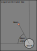
\includegraphics[width=.5\textwidth]{pictures/testbeam.pdf}
    	\caption{Schematic of the 2019 TestBeam setup at \ac{DESY} \cite{HANEL}. A laser beam was used to measure the \ac{WOM} detector response at beam angles spanning a \SI{90}{\degree} interval.}
    	\label{fig:testbeam-setup}
    \end{figure}
    
    We observe the following: For an incidence angle difference of about \SI{90}{\degree}, the $\overline{\Phi_{ew}}$ values show a difference of \SI{45}{\degree} in the TestBeam setup (see figure \ref{fig:hanel-phi}). In the cosmics experiment, four values for a \SI{90}{\degree} angular difference can be gathered: Between positions C-2 and L-0, L-0 and C-1, C-1 and R-0, and R-0 and C-2. The $\overline{\Phi_{ew}}$ differences here are about \SI{28}{\degree}, \SI{74}{\degree}, \SI{9}{\degree} and \SI{54}{\degree} respectively, putting all except one in the same order of magnitude observed in Hanel's thesis.
    Comparing the standard deviations between the experiments, we observe consistency once again: Both the ones measured in the TestBeam experiment, as well as the ones in the cosmics setup, lie in the range of about 40 to \SI{70}{\degree}, as evident in figure \ref{fig:hanel-std}.
    
    \begin{figure}
    	\centering
    	
    Mean angle measured in TestBeam experiment	
    
    	\begin{subfigure}{\textwidth}
    		\centering
    		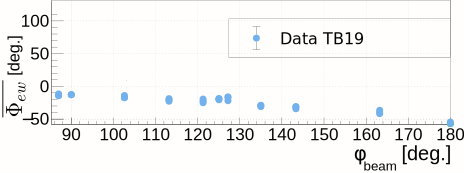
\includegraphics[width=.75\textwidth]{pictures/hanel_phi-ew.pdf}
    		\caption{}
    		\label{fig:hanel-phi}
    	\end{subfigure}
    \vspace{.5cm}
    
    Standard deviation of mean angle measured in TestBeam experiment
    
	    \begin{subfigure}{\textwidth}
	    	\centering
	    	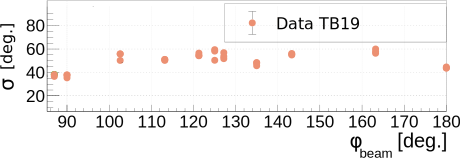
\includegraphics[width=.75\textwidth]{pictures/hanel_phi-std.pdf}
	    	\caption{}
	    	\label{fig:hanel-std}
	    \end{subfigure}
    \caption{Results from TestBeam experiment presented in Hanel's bachelor's thesis. Adapted from \cite{HANEL}.}
    \end{figure}
    
    
    Given the fact that even for an incidence angle difference of \SI{90}{\degree} the $\overline{\Phi_{ew}}$ values show variations in the same order as or even smaller than their standard deviations, it is for the moment impossible to assign the $\phi_{ew}$ of a singular event to a certain $\overline{\Phi_{ew}}$, thereby determining its location. To do this, the precision of the $\overline{\Phi_{ew}}$ values would need to be increased greatly. While this has already been discussed for the TestBeam experiment in Hanel's thesis, it should be mentioned here that the results from the cosmics setup suggest that the influences of the optical coupling of the detectors to the \ac{WOM} tube appears to make even the distinction between a \SI{90}{\degree} incidence position difference impossible for one side of the \ac{WOM}, as shown in the $\overline{\Phi_{ew}}$ difference for positions C-1 and R-0, which is only \SI{9}{\degree}. 
    
    The non-uniformity in the optical coupling, as shown in figure \ref{fig:phi-ew_C0}, would need to be analysed in detail to account for it when evaluating $\phi_{ew}$ values of singular events. It seems to suggest that for the cosmics setup, light seems to be primarily detected by channels 0 and 1, which could be caused by the optical gel as mentioned above, but could also be linked to a non-perfect coverage of the \ac{WOM} tube by the \ac{SiPM} array. This could be caused by a shift of one of the components away from the central position, as illustrated in figure \ref{fig:wom-shift}. A slightly elliptical tube would not match the \ac{SiPM} array on the \ac{PCB} either, and hinder the detection of photons in most channels.
    
    \begin{figure}[h]
    	\centering
    	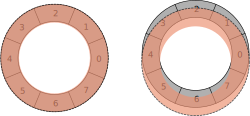
\includegraphics[width=.7\textwidth]{pictures/coverage.pdf}
    	\caption{Example of ideal coverage (left) and imperfect coverage (right) of \ac{SiPM} (grey) array on \ac{WOM} (orange) due to a shift between the structures.}
    	\label{fig:wom-shift}
    \end{figure}
    
    However even knowing the exact influence of optical coupling and tube imperfections, the method of determining en event's location used in this experiment is likely to cause increased standard deviations in the $\overline{\Phi_{ew}}$ values: Due to the fact that cosmic muons were used to record events in the \ac{LS} detector box, measurement runs took several days to measure a statistically significant number of events. While filtering events for certain positions, compromises had to be made between the number of events still left after the cut, and the accuracy to which the measurement location was set. Thus, to keep a reasonable number of events in the cut, the positions were given by an interval each, smearing out the incidence location angle, and decreasing the accuracy of the $\overline{\Phi_{ew}}$ value of each position. To combat this, one would probably need to use a setup such as the TestBeam again, which lets the experimentalist control the number of events and their locations to a higher degree.
    
    




    
    

\section{Pickup Signals}

    As mentioned above, the measurement runs were conducted over the course of several days. While taking measurements during May 2021, we noticed the recorded signals to show unusual behaviour starting in the evening of May 5th. Instead of the usual waveforms caused by a muon event, more than \SI{90}{\percent} of recorded 'events' looked like they were entirely made of noise. A waveform of such a 'pickup event', as they were later dubbed, can be seen in figure \ref{fig:pickup}. The pickup events dominated the recorded data for the entirety of May and the first half of June, making regular data taking impossible. During this time, it was attempted to identify the cause and source of the pickup events, but no specific technical cause could be identified. On the day the pickup events were first spotted the only less than 'ordinary' environmental factor identified was a thunderstorm that occurred that same afternoon. Starting June 22nd the pickup events stopped dominating the signals for unknown reasons, and regular measurements were continued.
    
    % FIGURE waveform pickup \ac{SiPM} and \ac{PMT}
    
    \begin{figure}[h!]
        \centering
        \begin{subfigure}{.5\textwidth}
        \centering
          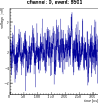
\includegraphics[width=.9\textwidth]{pictures/pickup_wave_sipm.pdf}
          \caption{}
          \label{fig:pickup-sipm}
        \end{subfigure}%
        \begin{subfigure}{.5\textwidth}
        \centering
          \includegraphics[width=\textwidth]{pictures/pickup_wave_pmt.pdf}
          \caption{}
          \label{fig:pickup-pmt}
        \end{subfigure}
        \caption{Pickup event waveform as seen in the a) \acsp{SiPM} and b) \acsp{PMT}. While in the \ac{SiPM} only noise was recorded, the trigger channels such as channel 8 as here illustrated show a notable variation in voltage from the noise levels, which were then used to filter these events.}
        \label{fig:pickup}
    \end{figure}
    
    The data taken during May and June was analysed to attempt to salvage regular events. We noticed that we could distinguish pickup from regular events by filtering on the amplitude of the trigger \acsp{PMT} - the waveforms looked very similar in all 4 trigger channels, with the notable feature of the \acsp{PMT} showing relatively large positive signal values, which did not happen in a normal event. Additionally, the light yield calculated in the integration time was significantly lower than that of a muon event, however to prevent accidentally cutting muon events that happened to have a low light yield, events were filtered only by \ac{PMT} amplitudes.
    After applying the cuts on the \ac{PMT} amplitudes, we noticed that the pickup events have actually always been present, albeit with a significantly lower rate. This can be observed when comparing light yield histograms for a run with pickup events filtered, with the same run with no filter applied (see figure \ref{fig:pickup-filter}). The filtered histogram shows fewer entries in the near-zero region of light yield values. 
    
    % FIGURE light yield histogram with vs without pickup filter
    
    \begin{figure}[h!]
        \centering
        Light yield channel 0, data from 12th to 18th of April
        \begin{subfigure}{.5\textwidth}
        \centering
        \includegraphics[width=\textwidth]{pictures/integrals_nocut_12to18_2.pdf}
        \caption{}
        \label{fig:integral-nocut}
        \end{subfigure}%
        \begin{subfigure}{.5\textwidth}
        \centering
        \includegraphics[width=\textwidth]{pictures/integrals_cut_12to18_2.pdf}
        \caption{}
        \label{fig:integral-cut}
        \end{subfigure}
        \caption{Light yield measured in \ac{SiPM} channel 0 without a) and with b) pickup filtering active. With the filter active, a few events with a light yield of nearly \SI{0}{\volt\nano\second} were filtered out.}
        \label{fig:pickup-filter}
    \end{figure}
    
    
    To get an overview for the timeline of the strange behaviour of the experiment, runs from April and the end of June were also considered: In figure \ref{fig:pickup-timeline} the ratio $R$ of pickup to normal events is plotted for runs spanning the 12th of April until the 25th of June.
    
    \begin{align}
        R = \frac{\text{Number of pickup events}}{\text{Number of muon events}}
    \end{align}
    
    Here we can see that while the runs during May and the beginning of June consist mainly of pickup events, the ratio in April was never actually 0. 
%    Here we can also see that no significant difference in the pickup-non-pickup ratio can be seen between day and night runs.
    
    \begin{figure}
        \centering
        \includegraphics[width=\textwidth]{pictures/pickup-timeline.pdf}
        \caption{Pictured is the ratio of pickup to non-pickup events over the time span of 12th of April to the 25th of June 2021. Yellow spots indicate values for daylight measurements, blue ones the ones for night-time measurements. The first day where the pickup signals were noticed is marked with a grey vertical line. The ratio was kept under surveillance for data sets taken after this time as well, but continued in the same manner as the latest June measurements.}
        \label{fig:pickup-timeline}
    \end{figure}
    
    